%!TeX root = ./../MusterAbschlussarbeit.tex

%##########################################################
% Inhalt
%##########################################################

\clearpage
\chapter{Präsentation der Ergebnisse}

Um den Lernprozess evaluieren zu können, wurden verschiedene Experimente durchgeführt. Diese Experimente werden in diesem Kapitel vorgestellt und ausgewertet. 
Im folgenden Kapitel wird oft von dem trainierten Agenten gesprochen. Damit ist ein Modell gemeint, welches 25 Millionen Trainingsschritte auf dem schwarzen Spielfeld durchgeführt hat. Dies wird in \ref{fig:Vorlage} dargestellt. Dies entspricht etwa 830k gespielten Spielen.

\newpage
\section{Agent mit zusätzlichen Belohnungen}
In diesem Versuch bekam der Agent, zusätzlich zu den ursprünglichen Rewards, weitere Belohnungen für bestimmte Aktionen. Diese Belohnungen sollten den Agenten zu komplexeren Spielzielen leiten, um so schneller zu einer optimalen Policy zu gelangen.
In \ref{tab:rewards2} sind alle zusätzlichen Rewards ersichtlich. In diesem Versuch wurde 2.4Mio Spielzüge ausgeführt. Es stellte sich, trotz geringer Anzahl an Lernschritten, ein negatives Ergebnis herraus. Deshalb wurde auf ein längeres Training verzichtet.  

\begin{table}[!h]
    \centering
    \begin{tabular}{|c|c|}
    \hline
    \textbf{Aktion} & \textbf{Erhaltene Belohnung} \\
    \hline
    Abkreuzen von Feldern & 0.02f pro Feld \\
    \hline
    Abkreuzen eines gesamten Clusters & 0.04f pro Feld \\
    \hline
    Wahl eines Würfelpaars ohne legale Züge & -50.0f \\
    \hline
    Wahl eines Jokers ohne verfügbare Joker & -50.0f \\
    \hline
    \end{tabular}
    \caption{Zusatzbelohnungen für verschiedene Aktionen}
    \label{tab:rewards2}
\end{table}



Die  Grafiken \ref{fig:average_points} und \ref{fig:average_rewards} zeigen deutlich, dass je länger das Training voranschritt, die durchschnittlich erreichten Punkte pro Spiel sanken.
Die zusätzlichen Belohnungen führten dazu, dass der Agent nicht versuchte Spalten abzukreuzen oder Farben komplett auszufüllen. Dieser hielt das Abkreuzen von Clustern für deutlich effizienter, um seine Belohnungen zu maximieren, obwohl die Belohnungen für erreichte Spalten oder komplett ausgefüllte Farben mehr Punkte ergaben. Dies spricht dafür, dass in diesem Versuch Belohnungsumgehung aufgetreten ist. Verhindert werden könnte dies, indem dem Agenten die Exploration erleichtert wird. Beispielhaft kann die Anzahl der Spielzüge vergrößert werden.
Eine verlängerte Spieldauer hätte zur Folge, dass größere Teile des Spielfeldes ausgefüllt werden, wodurch der Agent komplexere Belohnungen erreichen und erlernen kann. 
\begin{figure}[!h]
    \centering
    \includegraphics[scale=0.6]{Bilder/average_points.png}
    \caption{Durchschnittliche Punkte des Agenten mit Zusatzbelohnungen}
    \label{fig:average_points}
\end{figure}

\begin{figure}[!h]
    \centering
    \includegraphics[scale=0.6]{Bilder/average_rewards.png}
    \caption{Durchschnittliche Belohnungen des Agenten mit Zusatzbelohnungen }
    \label{fig:average_rewards}
\end{figure}
\clearpage

\section{Vergleich trainiert und untrainiert}
In diesem Experiment werden die erreichten Punkte und Rewards eines untrainierten Agenten gegenüber den erzielten Ergebnissen eines trainierten Agenten gestellt. Der untrainierte Agent trainiert ein neu initialisiertes NN, welches zufällig gewählte Kantengewichte zwischen den Neuronen erhält. Um den Lernfortschritt zu bewerten, wurden eine Million Spielzüge von beiden Agenten ausgewertet. Beide nutzten das schwarze Spielfeld, welches in \ref{fig:Vorlage} dargestellt wurde, als Lernumgebung. 
Wie an den Grafiken \ref{fig:untrained_rewards} und \ref{fig:untrained_points} zu erkennen ist, hat der trainierte Agent tatsächlich einen höheren Durchschnitt an erzielten Punkten pro Spiel. Auch die gesammlten Rewards sind bei dem trainierten Agenten höher.
Dies liegt daran, dass die Rewards so festgelegt sind, dass der Agent sie nur erhält, wenn er auch im Spiel punktet.
Schon während des Trainings war ein merklicher Unterschied festzustellen, deshalb war das Ergebnis dieses Experiments zu erwarten.


\begin{figure}[!h]
    \centering
    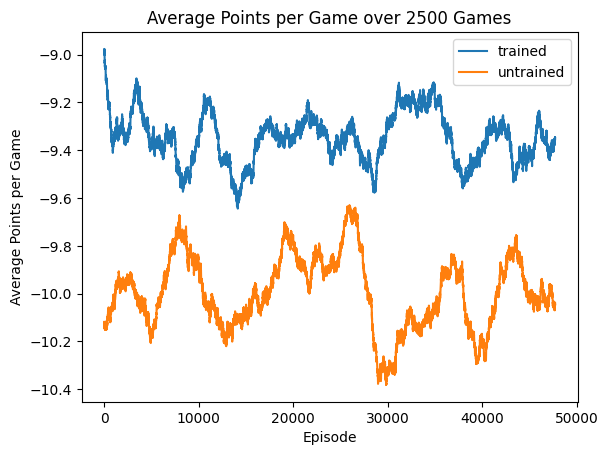
\includegraphics[scale=0.6]{Bilder/points_trained_vs_untrained.png}
    \caption{Durchschnitt der erreichten Punkte pro Spiel }
    \label{fig:untrained_points}
\end{figure}
\begin{figure}[!h]
    \centering
    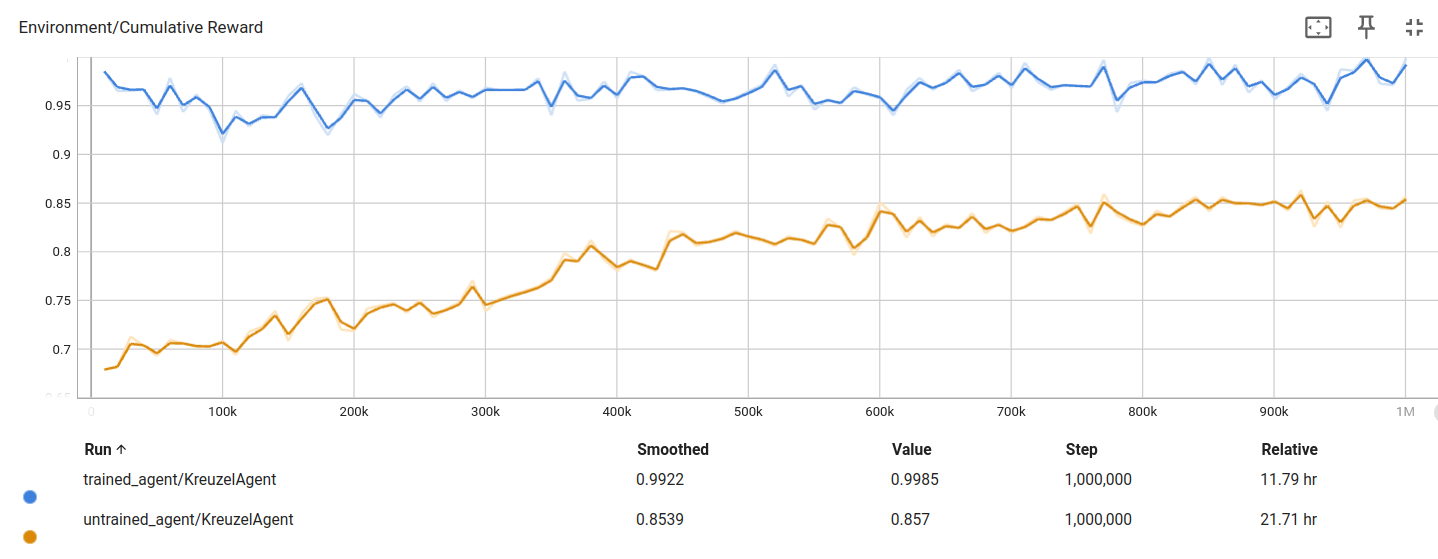
\includegraphics[scale=0.3]{Bilder/rewards_untrained.png}
    \caption{Übersicht der gesammelten Belohnungen}
    \label{fig:untrained_rewards}
\end{figure}

\newpage
\section{Training auf Sonderfeldern}
In diesem Experiment wurden die erreichten Puntke und Rewards des trainierten Agenten gegen einen Agenten, welcher mit Sonderfeldern trainiert wurde verglichen. Beide Agenten wurden mit dem selben vortrainierten Modell instanziiert. Dieser Versuch sollte überprüfen, ob ein Agent im Verlauf besser erlernen kann, welche Stellen im Beobachtungsvektorvektor für welche Information zuständig sind. 

\begin{figure}[!h]
    \centering
    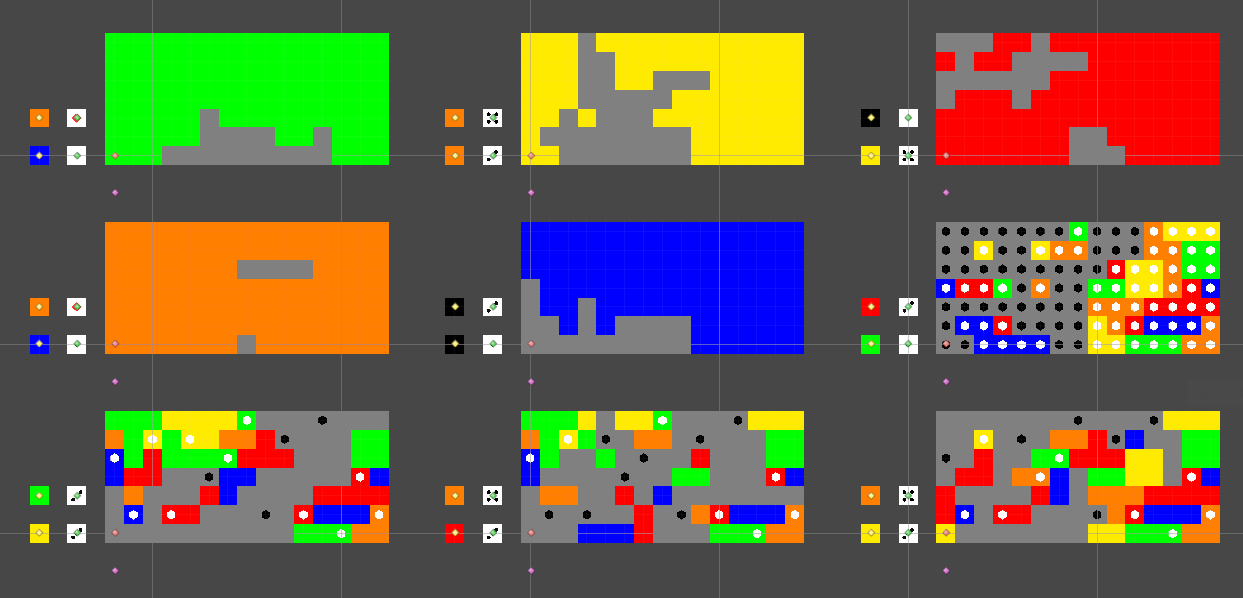
\includegraphics[scale=0.4]{Bilder/specialFields.png}
    \caption{Übersicht der speziellen Felder}
    \label{fig:specialFields}
\end{figure}

In der Grafik \ref{fig:specialFields} ist das Trainingumfeld mit den speziellen Feldern dargestellt. Jedes der Felder hat gewisse Besonderheiten, welche sich von den normalen Spielfeldern abgrenzen.
Fünf Felder sind in einer kompletten Farbidentität eingefärbt. In \ref{lst:DiceShift} wurde der Zahlenwürfel manipuliert, um häufiger die entsprechende Farbe zu werfen. Diese Felder sollten dem Agenten besser den Zusammenhang des Farbwürfels und des gewählten Farbidentität der Kästchen näherbringen.
In dem anderen Spielfeld ist jedes Feld als Sternfeld markiert. Dies sollte dem Agenten zeigen, dass jedes Feld mit markierten Sternen mehr Punkte bringt.
Bei den anderen drei Feldern ist jedes Feld von vornherein als verfügbar markiert. Dies sollte zum einen das Konzept des verfügbaren Feldes vermitteln, zum anderen dem Agenten ermöglichen das Feld weiter als normal zu explorieren, um die komplexen Ziele des Spiels leichter zu erreichen. \\
Aus der Grafik \ref{fig:special_points} lässt sich ableiten, dass das Modell, welches mit speziellen Feldern trainiert wurde, im Durchschnitt weniger Punkte erreichte, als der normal trainierte Agent. Dieses Training führte nicht zu einer Verbesserung des Modells. Ursache hierfür liegt sicher im Spielfeld, in welchem alle Felder als Sternfelder markiert wurden. Hier konnte der Agent willkürlich Züge ausführen und bekam überdurchschnittlich viele Punkte. Deshalb priorisierte der Agent nicht mehr die eigentlichen Ziele, was wiederum zur Folge hatte, dass die Leistung des Agenten auf dem eigentlichen Feld schlechter wurde. 

\begin{figure}[!h]
    \centering
    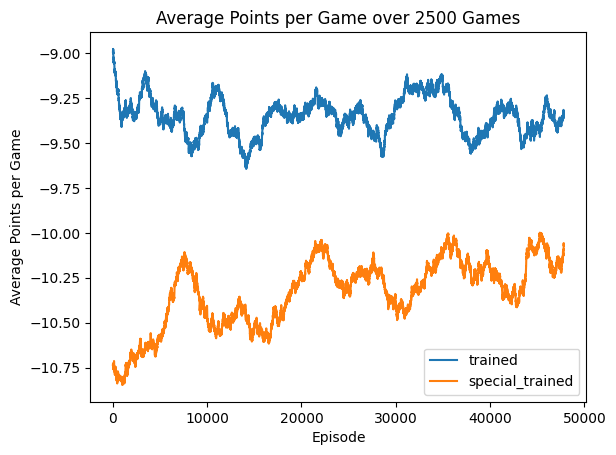
\includegraphics[scale=0.6]{Bilder/points_special_trained.png}
    \caption{Durchschnitt der erreichten Punkte beider Agenten}
    \label{fig:special_points}
\end{figure}

 \newpage
\section{Training mit mehr Spielzügen}

In diesem Experiment trainierte der Agent mit mehr zur Verfügung stehenden Spielzügen. Dadurch konnte der Agent das Feld besser explorieren und mehr Aktionen auslösen, welche zu Belohnungen führten. Dies hat zur Folge, dass auch schwierig erreichbare Rewards ausgelöst wurden, welche somit vom Agent erlernt werden konnten. 
Die Grafik \ref{fig:turns_points} zeigt, dass das Experiment eine Verbesserung des Models zur Folge hatte, da im Durchschnitt etwas mehr Punkte erreicht wurden.

\begin{figure}[!h]
    \centering
    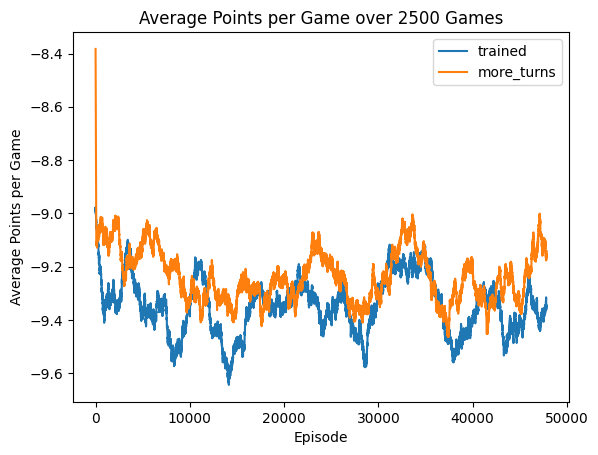
\includegraphics[scale=0.6]{Bilder/points_more_turns.png}
    \caption{Vergleich 'Mehr Züge' und 'trainierter Agent'}
    \label{fig:turns_points}

\end{figure}

\newpage
\section{Überprüfung auf Überanpassung}
In diesem Experiment sollte der Agent auf Überanpassung überprüft werden. Trainierter und untrainierter Agent spielten das Spiel nach normalen Spielregeln auf einem anderen Spielfeld.
\ref{fig:OrangeField} zeigt die angepasste Trainingsumgebung. Das Spielfeld wurde dem orginalen Spiel nachempfunden. Beide Agenten trainierten 1 Mio. Lernschritte, wobei erreichte Punkte und Belohnungen aufgezeichnet wurden.
In den Grafiken \ref{fig:orange_points} und \ref{fig:orange_rewards} ist erkennbar, dass beide Agenten ungefähr die selben Rewards gesammelten haben. Der untrainierte Agent konnte im Durchschnitt jedoch etwas mehr Punkte sammeln.
Dies schließt darauf, dass der Agent tatsächlich nur auf dem im Training verwendeten Spielfeld gut performen kann und neue Spielfelder erst erlernen muss.
Interessant ist weiterhin, dass der Durchschnitt aller Punkte etwa 2 Punkte über dem des anderen Spielfeldes liegt, was auf eine höhere Schwierigkeit des schwarzen Spielfeldes hinweist.

\begin{figure}[!h]
    \centering
    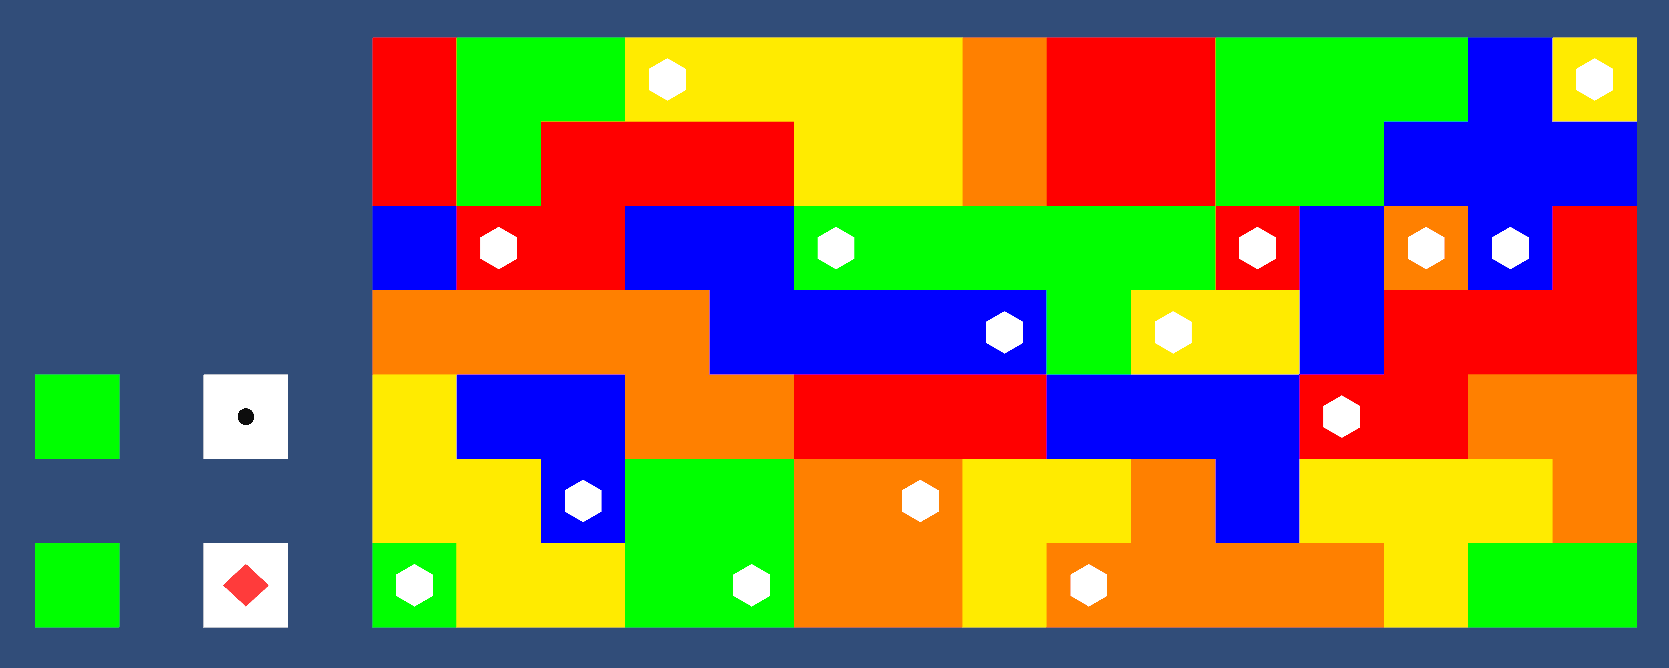
\includegraphics[scale=0.2]{Bilder/OrangeField.png}
    \caption{Trainingsumgebung für das Training auf dem orangenem Feld}
    \label{fig:OrangeField}
\end{figure}

\begin{figure}[!h]
    \centering
    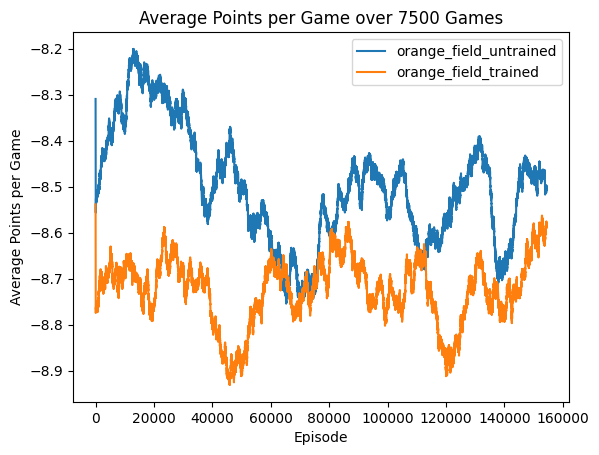
\includegraphics[scale=0.6]{Bilder/points_orange_field.png}
    \caption{Vergleich Punkte 'trainiert' und 'untrainiert' auf orangen Spielfeld}
    \label{fig:orange_points}
\end{figure}
\begin{figure}[!h]
    \centering
    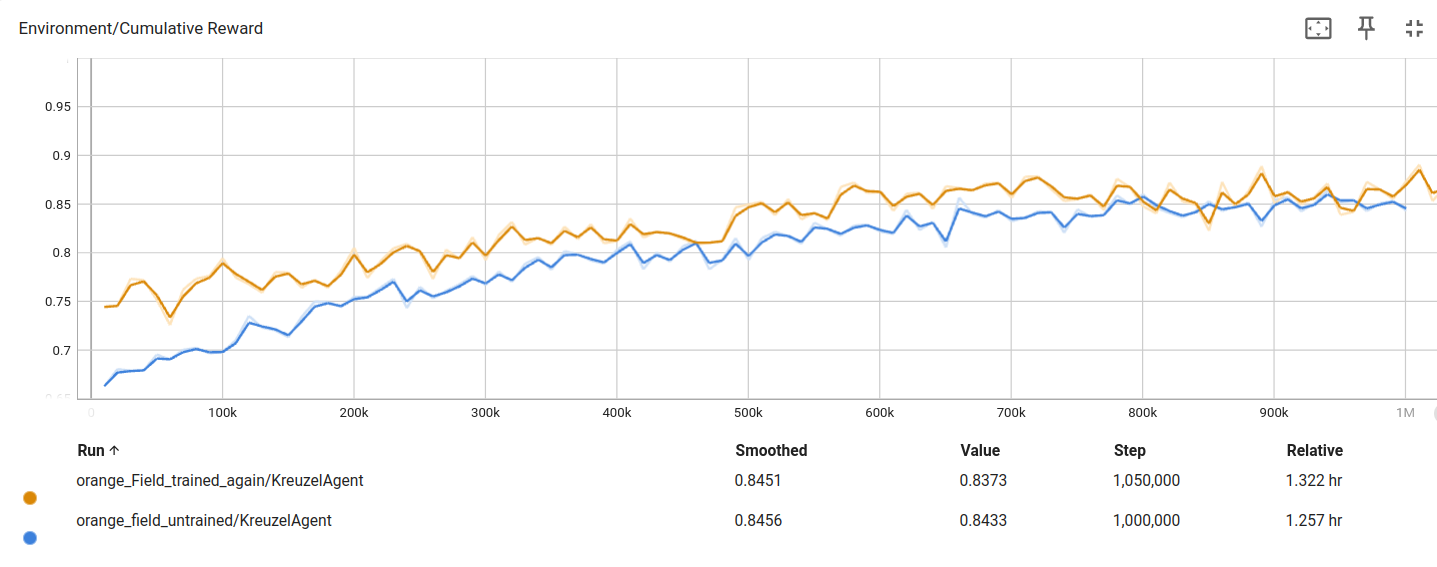
\includegraphics[scale=0.3]{Bilder/rewards_orange_field.png}
    \caption{Übersicht gesammelte Rewards auf orangen Spielfeld}
    \label{fig:orange_rewards}

\end{figure}

\newpage
\section{Training auf Minifeld}
Um zu überprüfen, ob ein kleineres Feld  einen positiven Effekt auf das Training hat, wurde ein Spielfeld um 3 Zeilen gekürzt und fungierte als Trainingsumgebung. \ref{fig:miniFeld} zeigt das angepasste Spielfeld. Im Anschluss wurde die Leistung des Agenten auf dem normalen Spielfeld gegenüber dem Ergebnis eines untrainierten Agenten gestellt.  Beide Agenten wurde mit einem neuen NN initialisiert.
Da die Beobachtungen von Modellen gleich bleiben müssen, wurden nicht mehr vorhandene Kästchen mit Nullen im Vektor präsentiert. \ref{lst:PushEmptyField} zeigt den Quellcode zum Übergeben eines leeren Feldes.

\lstinputlisting[language=csh, label={lst:PushEmptyField}, caption={Befüllen des Beobachtungsvektor mit leerem Feld}]{Programmcode/PushEmptyField.cs}

\begin{figure}[!h]
	\centering
	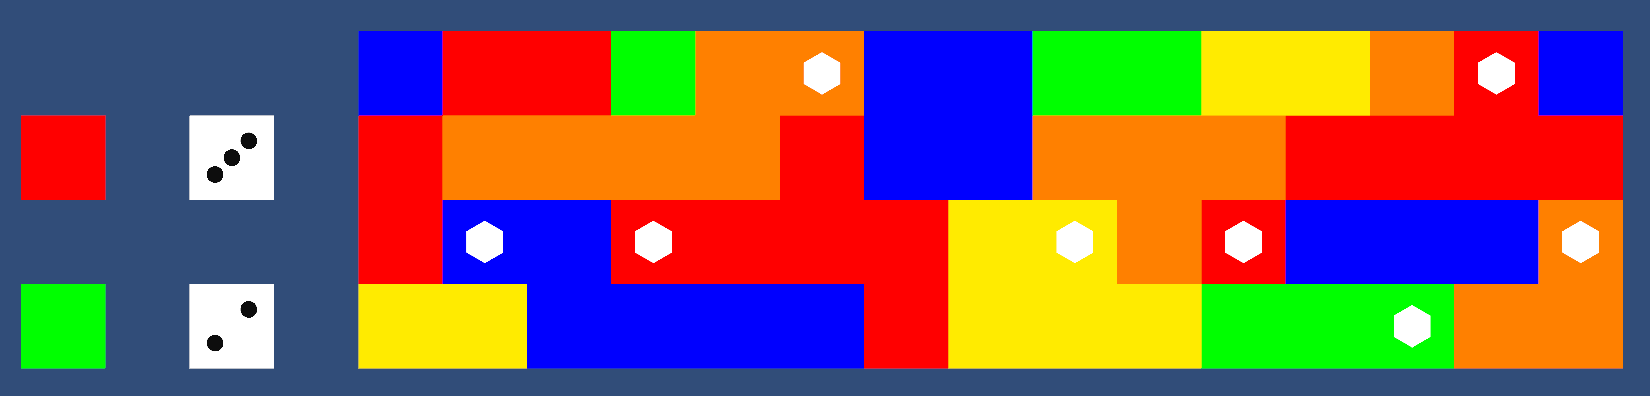
\includegraphics[width=0.5\textwidth]{Bilder/miniFeld.png}
	\caption{Lernumgebung für einen Agenten auf dem 'MiniFeld'}
	\label{fig:miniFeld}
\end{figure}
\newpage

Die Grafiken \ref{fig:Minifeld_rewards} und \ref{fig:Minifeld_points} zeigen den Durchschnitt der erreichten Punkte pro Spiel und die gesammelten Blohnungen während des Trainings.
Es wird ersichtlich, dass der mit einem kleinen Feld vortrainierte Agent schlechter performt, als die beiden anderen. Belohnungen wurden auch hier nur verteilt, wenn es zur Punktewertung kommt. Deshalb ist es interessant, dass der untrainierte Agent mehr Punkte erreicht, als der auf dem kleinen Feld vortrainierte Agent, obwohl dieser wiederum einen höheren Durchschnitt an Belohnungen erhält. 

Ursache für das schlechtere Ergebnis ist auf die Überanpassung zurückzuführen. So wurde beim Training auf dem kleinen Feld ausschließlich dieses  angepasste Feld erlernt und nicht eine gute Spielweise. Weiterhin konnte der auf dem kleineren Feld trainierte Agent nicht den kompletten Beobachtungsvektor erlernen, da ein großer Teil leer übergeben wurde.


\begin{figure}[!h]
    \centering
    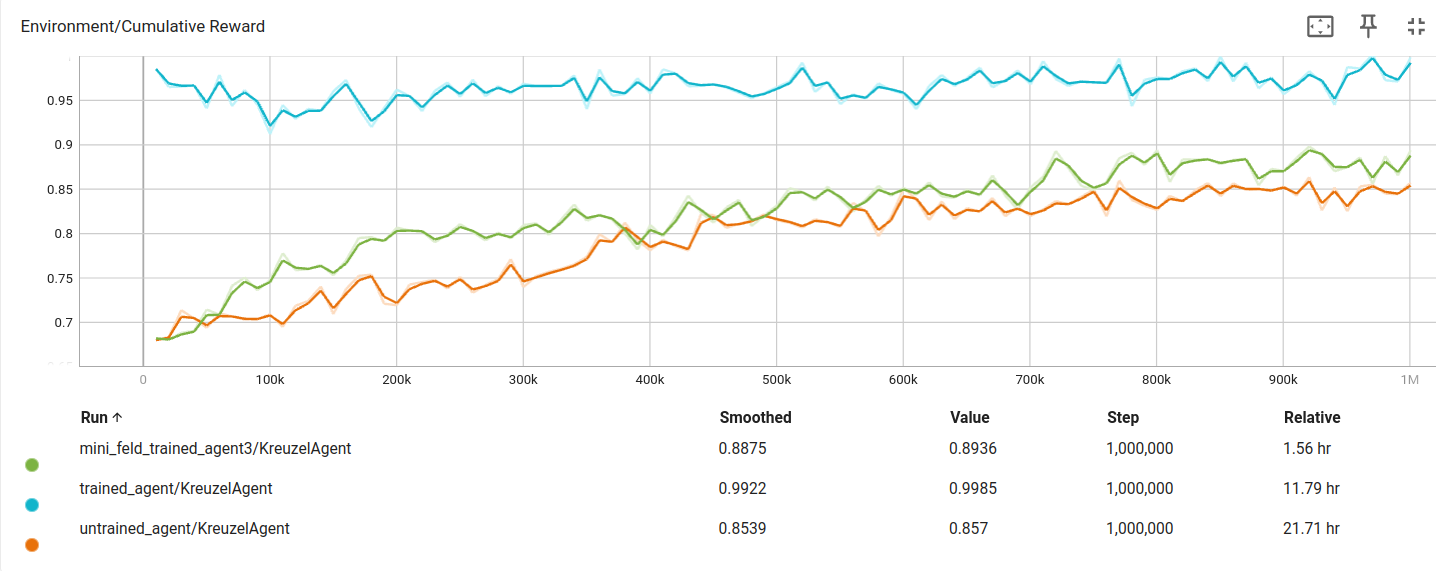
\includegraphics[scale=0.3]{Bilder/rewards_minifield.png}
    \caption{Gesammelte Belohnungen mit Minifeld}
    \label{fig:Minifeld_rewards}
\end{figure}

\begin{figure}[!h]
    \centering
    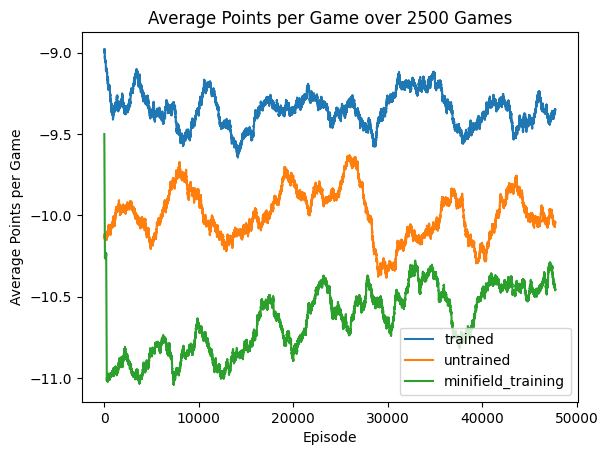
\includegraphics[scale=0.5]{Bilder/points_minifeld.png}
    \caption{Vergleich erreichte Punkte}
    \label{fig:Minifeld_points}
\end{figure}

\clearpage
\section{Training blinder Agent}
In diesem Experiment wurden dem blinden Agenten lediglich die Würfel, die Anzahl der verbleibenden Joker und die aktuelle Runde des Spiels übergeben.
Dieser Versuch sollte zeigen, wie gut ein Agent, der die aktuelle Informationen vom  Spielfeld nicht erhält, perfomt. Dies sollte überprüfen, ob das trainierte Modell tatsächlich besser ist, als eine rein zufällige Spielweise.
Da die Auswahl der Felder durch zufällige Interpolation aller möglichen Felder abläuft, kann der blinde Agent normal spielen. Durch den Versuchsaufbau verringert sich der Beobachtungsvektor von 916 auf eine Größe von 15 Informationen. Dies führte dazu, dass der Agent schnell zu seiner optimalen Policy gelangen konnte. Auch wenn der Agent das Spielfeld nicht übergeben bekommt, kann er dieses implizit erlernen. Dieser Prozess wäre allerdings nicht sonderlich robust, sehr lernintensiv und würde nicht auf anderen Feldern funktionieren. \\ 
Der Agent konnte bereits nach sehr kurzer Zeit von etwa 400k Lernschritten gegen sein Maximum konvergieren, wie in \ref{fig:onlydice_rewards} ersichtlich ist. Dort schneiden sich die beiden grünen Graphen und verbleiben auf ungefähr dem selben Niveau. Dieses Modell wurde insgesamt 5 Mio. Episoden trainiert. Der trainierte Agent konnte sich dagegen kontinuierlich minimal verbessern und erreichte auch nach 25Mio Lernschritten noch keinen Maximalwert. \\
Abbildung \ref{fig:onlydice_points} zeigt, dass auch der blinde Agent im Durchschnitt weniger Punkte erreichen konnte. Dies beweist, dass das Training, trotz der geringen erreichten Punkte, positiv verlaufen ist.


\begin{figure}[!h]
    \centering
    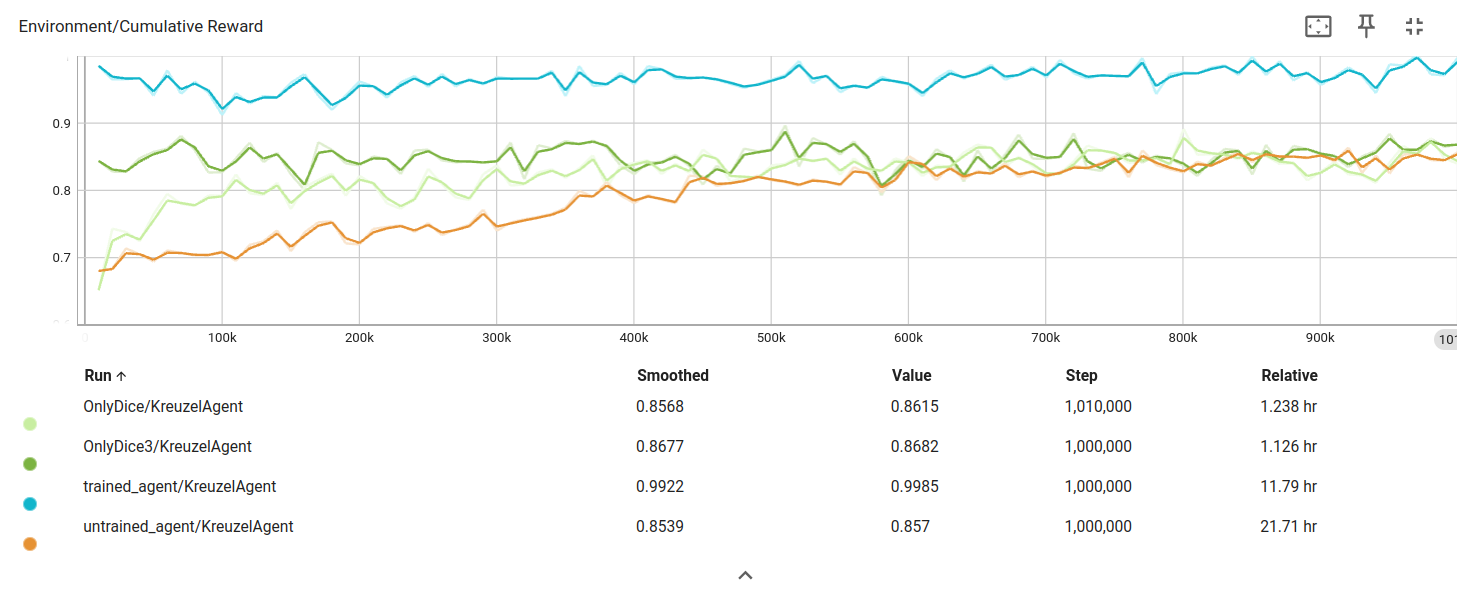
\includegraphics[scale=0.3]{Bilder/rewards_onlydice.png}
    \caption{Gesammelte Belohnungen blinder Agent}
    \label{fig:onlydice_rewards}
\end{figure}

\begin{figure}[!h]
    \centering
    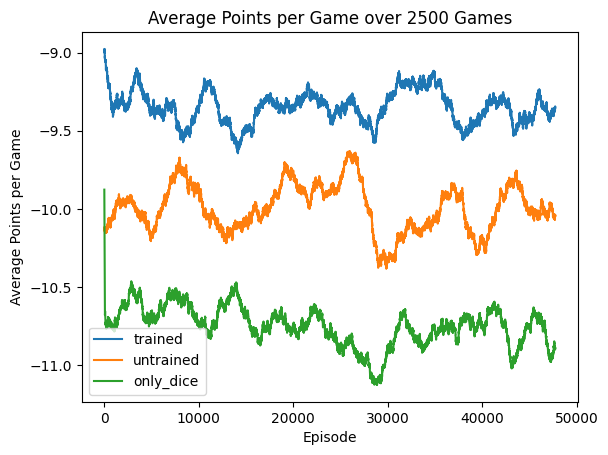
\includegraphics[scale=0.5]{Bilder/points_onlydice.png}
    \caption{Vergleich erreichte Punkte blinder Agent}
    \label{fig:onlydice_points}
\end{figure}